\chapter{Project Premise \& Model Design} 

%TODO: need to discuss ferry characteristics - task oriented

Any application running over a message ferrying network must have the following characteristics.

\begin{description}
\item[Delay Tolerance: ]
Since data is transported by a physical device, significant delays of minutes to hours must be expected.
\item[Loss Tolerance: ]
Given that ferries have limited memory, loss of data must be expected.
\item[Small and Independent Messages: ]
Following from the limited memory capacity of ferries and the high probability of packet loss, a reliable method for segmentation and reassembly of messages should not be expected. 
Applications should limit the size of messages such that the can be transmitted in their entirety using one network packet.
(See section \ref{sec:fountain_codes} for future work)
\end{description}

Given these criteria, a message ferrying network is unsuitable for many classic networking applications including web browsing, real-time voice or text communication and file transfer.
As such, a very specialized 'state monitoring' network designed for non-critical monitoring of remote sensors is considered.

\section{State Monitoring Network}

The general premise for this project consists of a network containing numerous, uniquely identifiable source nodes. 
Each source node has a limited number of properties, in the form of key/value pairs, specifying a property name (the key) and its current value.
Properties may change overtime and each change defines a new state for the source node.
A temperature sensor for example, might support a 'temperature' property, the value of which is the current temperature updated every hour.
Properties do not have to contain a single value and each may be as large as the payload limit of network packets. %Somewhat of a vague statement

%TODO: What is the ferry
%

\begin{figure}[h]
    \centering
    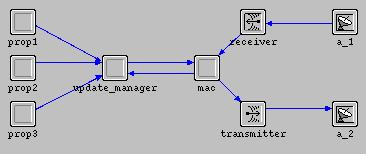
\includegraphics[width=.5\textwidth]{images/source}
    \caption{Source Node}
    \label{fig:source}
\end{figure}

\begin{figure}[h]
    \centering
    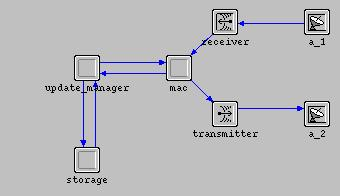
\includegraphics[width=.5\textwidth]{images/ferry}
    \caption{Ferry Node}
    \label{fig:Ferry}
\end{figure}

\begin{figure}[h]
    \centering
    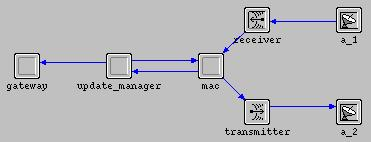
\includegraphics[width=.5\textwidth]{images/gateway}
    \caption{Gateway Node}
    \label{fig:Gateway}
\end{figure}

The network and message ferrying algorithm is designed to synchronize a central repository with the current state of every source node.
Only the most recent state (or most recent value) for each property is important, not the history of how that property has changed.
This limits the number of packets which can exist in the network as only the most recent update must be reported.
%The significance of this characteristic is described below. 
The message ferries collect data from source nodes when they are in range and transport it to the central repository.
The central repository is assumed to be a server connected to the Internet.
Ferries pass updates they have collected from source nodes to special gateway nodes.
These gateway nodes are then responsible for using a reliable delivery mechanism over a standard IP network to update the central repository.

\emph{Insert image showing this process.}

\section{Network Elements}

This section describes the elements present in the network.

\subsection{Physical Network Entities}

The network is comprised of four types of nodes.

\begin{description}
\item[Source Node: ] 
Static nodes in the network which have a set of properties (key/value pairs).
After a property of a source changes, known as a state change, it attempt to notify the central repository by transferring update packets to message ferries.
A source node could be, for example, a remote temperature sensor.
\item[Message Ferry: ] 
A mobile node which collects updates from source nodes when they are in range.
Message ferries store update packets from source nodes within a buffer. 
When in range, these update packets are forwarded to gateway nodes.
A source node could be, for example, a specially equipt cell phone or a small computer attached to a vehicle. 
\item[Gateway: ]
Gateway nodes download update packets form message ferries and forward them to the central repository over the Internet.
Transfer of updates between the gateway and central repository is assumed to be reliable. 
\item[Central Repository: ] 
The central repository is a server and the final destination for updates sent from source nodes.
It maintains a list of the current state of all source nodes.
There is only one central repository node.
\end{description}

\subsection{Inter-Node Communication}

Nodes communicate with each other using the ZigBee (802.15.4) MAC layer at 2.4 $GHz$. 

%TODO: citing
%TODO: More about 802.15.4

\subsection{Packets}

The ZigBee MAC layer uses special packets to establish and acknowledge inter-node communication.
At the network layer, two types of packets are used as follows:

\begin{description}
\item[Update Packet: ]
Update packets are generated by source nodes when a message ferry is in range and their state has changed. 
Source nodes will continue to generate update packets until the state change is acknowledged by the central repository (using an acknowledgment packet).
\item[Acknowledgment Packet: ] 
Packets sent from the central repository to source nodes acknowledging that the state update has been recorded.
\end{description}

\emph{Interim Report: There is more to this which I have not included.}